\documentclass[10pt]{beamer}

%STANDARD PREAMBLE
%https://tex.stackexchange.com/questions/68821/is-it-possible-to-create-a-latex-preamble-header
\usepackage{/Users/mwojno01/Research/Learning/latex_preamble/beamer_preamble}



%
%% ALLOW FOR ITEMIZE ENVIRONMENTS WITH NO PRECEDING
% SPACING, IF DESIRED
% Reference: https://tex.stackexchange.com/questions/86054/how-to-remove-the-whitespace-before-itemize-enumerate
%\usepackage{enumitem}% http://ctan.org/pkg/enumitem 
\usepackage{paralist}

\title{Unit tests in python}

\begin{document}

\maketitle

\section{Introduction}

\begin{frame}{Unit tests}
\alert{Unit tests} test that functions in the source code behave as expected. 

 For an example, see \href{https://github.com/mikewojnowicz/acc/blob/master/tests/unit/test_arithmetic.py}{\blue{here}}.
\end{frame}

\begin{frame}{Why write unit tests?}
\begin{itemize}
\item (Prototypical motivation) Ensure that if you change your source code later on, you don’t accidentally convert a working function into a buggy one.  %This basically takes the work most of us do anyways to test a function, and allows us to rerun automatic checks before committing. 
\item Illustrate usage of functions to other people (or to “future you”)
\item The requirement to test code often leads to better factored source code {\tiny (and sometimes even better factored underlying mathematical arguments in papers!)}  %Tell them the ELBO story — took ~ 1 week of my time, a couple hours of a PI’s time, and most of a meeting with 4 ppl with Ph.D.’s to find a couple of silly errors in the  ELBO.   Unit tests can prevent this — getting stuck on some tedious detail, lost in a sea of complexity!   
\item Can help check and reinforce your own understanding when learning something new. {\tiny [Is the function behaving like you expect?  If not, is there perhaps some gap in your understanding behind it — and so your mind (and therefore the code) needs to be tweaked?}    %Finally property-based unit tests can help check and reinforce your own understanding when you’re learning something new. Is the function behaving like you expect?  If not, is there perhaps some gap in your understanding behind it — and so your mind (and therefore the code) needs to be tweaked?  (Catchy motto: unit testing your mind).    Example: inverse wishart sampler… better understanding of the prior sum of squares parameter. 
\end{itemize}
	
\end{frame}


\section{Conventional unit testing}
\begin{frame}{Conventional unit testing}

In \alert{conventional unit testing}, you write tests that assert that a \textit{particular} input is transformed into a \textit{particular} answer known to be correct.
\vfill 
We will practice writing tests like this using the \texttt{catinabox} module.
\end{frame}


\section{Property-based testing}


\begin{frame}{Property-based testing}

In \alert{property-based testing}, you write tests that assert that something should be true for every case, not just the ones you happen to think of.
\vfill 
\begin{itemize}
\item \textbf{Conventional unit tests}: Assert that a \textit{particular} input is transformed to a \textit{particular} answer known to be correct.
\item \textbf{Property-based tests}: Assert that some property holds for \textit{all} data matching some specification.
\end{itemize}
\vfill 
\pause 
\metroset{block=fill}
\begin{block}{The \texttt{hypothesis} package}
\texttt{hypothesis} is a Python library supporting property-based testing.
\vfill
It works by generating arbitrary data matching your specification and checking that your guarantee still holds in that case.
\vfill
It can find edge cases in your code you wouldn’t have thought to look for.
\end{block}
\end{frame}


\begin{frame}
\begin{center}
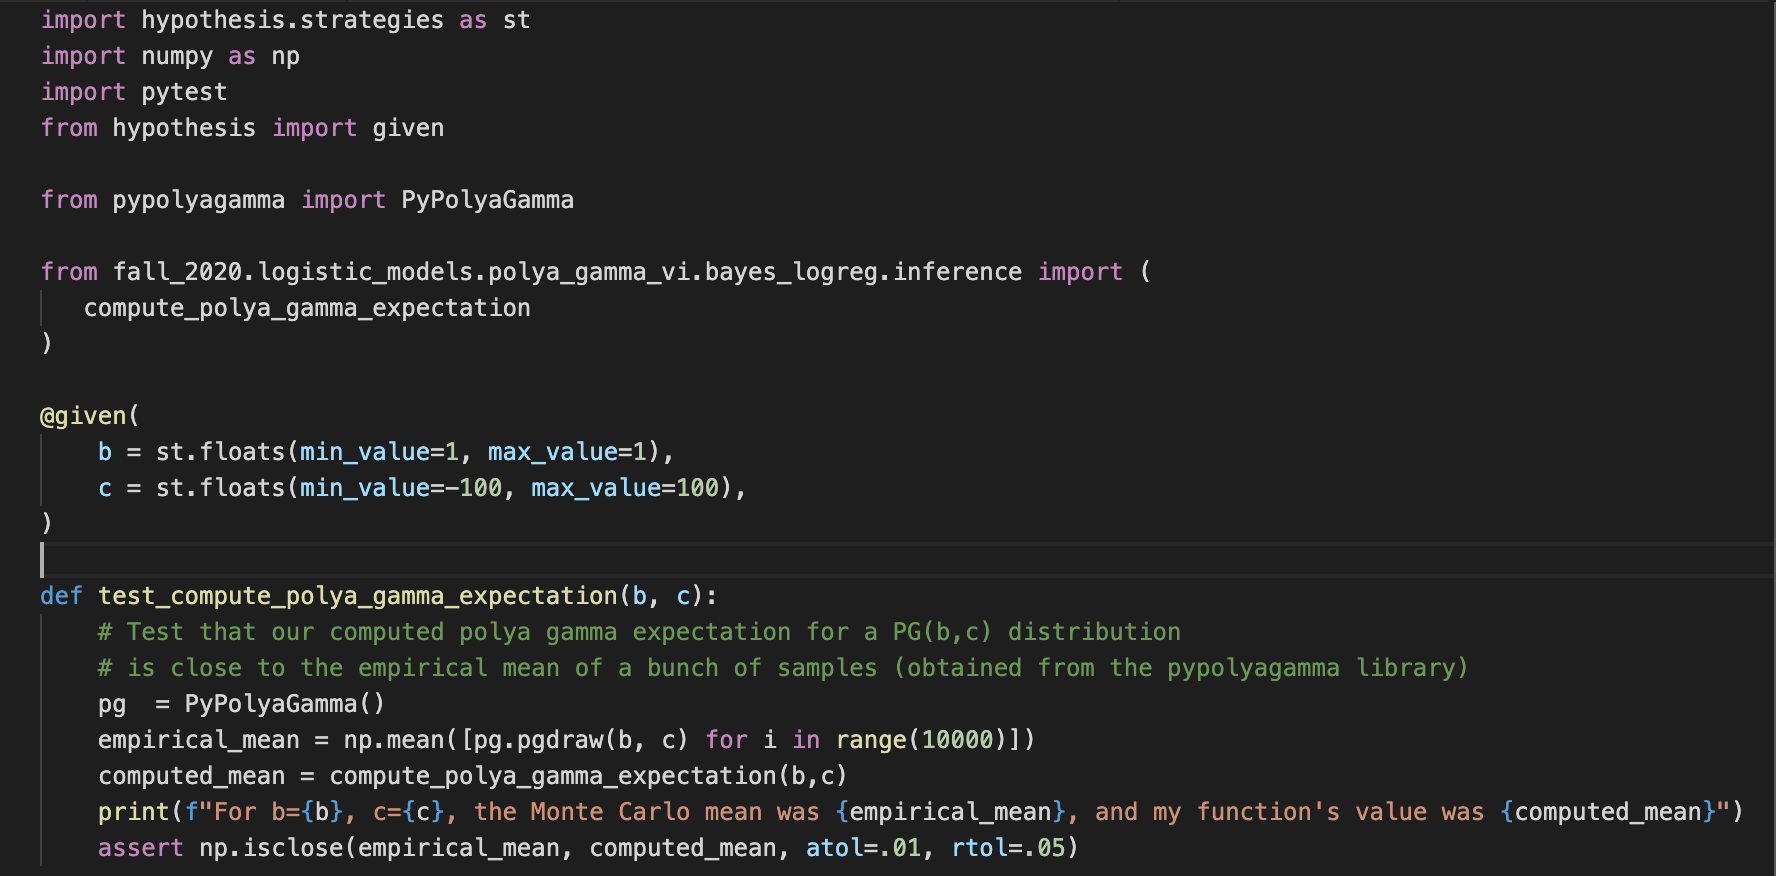
\includegraphics[width=\textwidth]{images/pypolyagamma_test}	
\end{center}
	
\end{frame}

\begin{frame}
\begin{center}
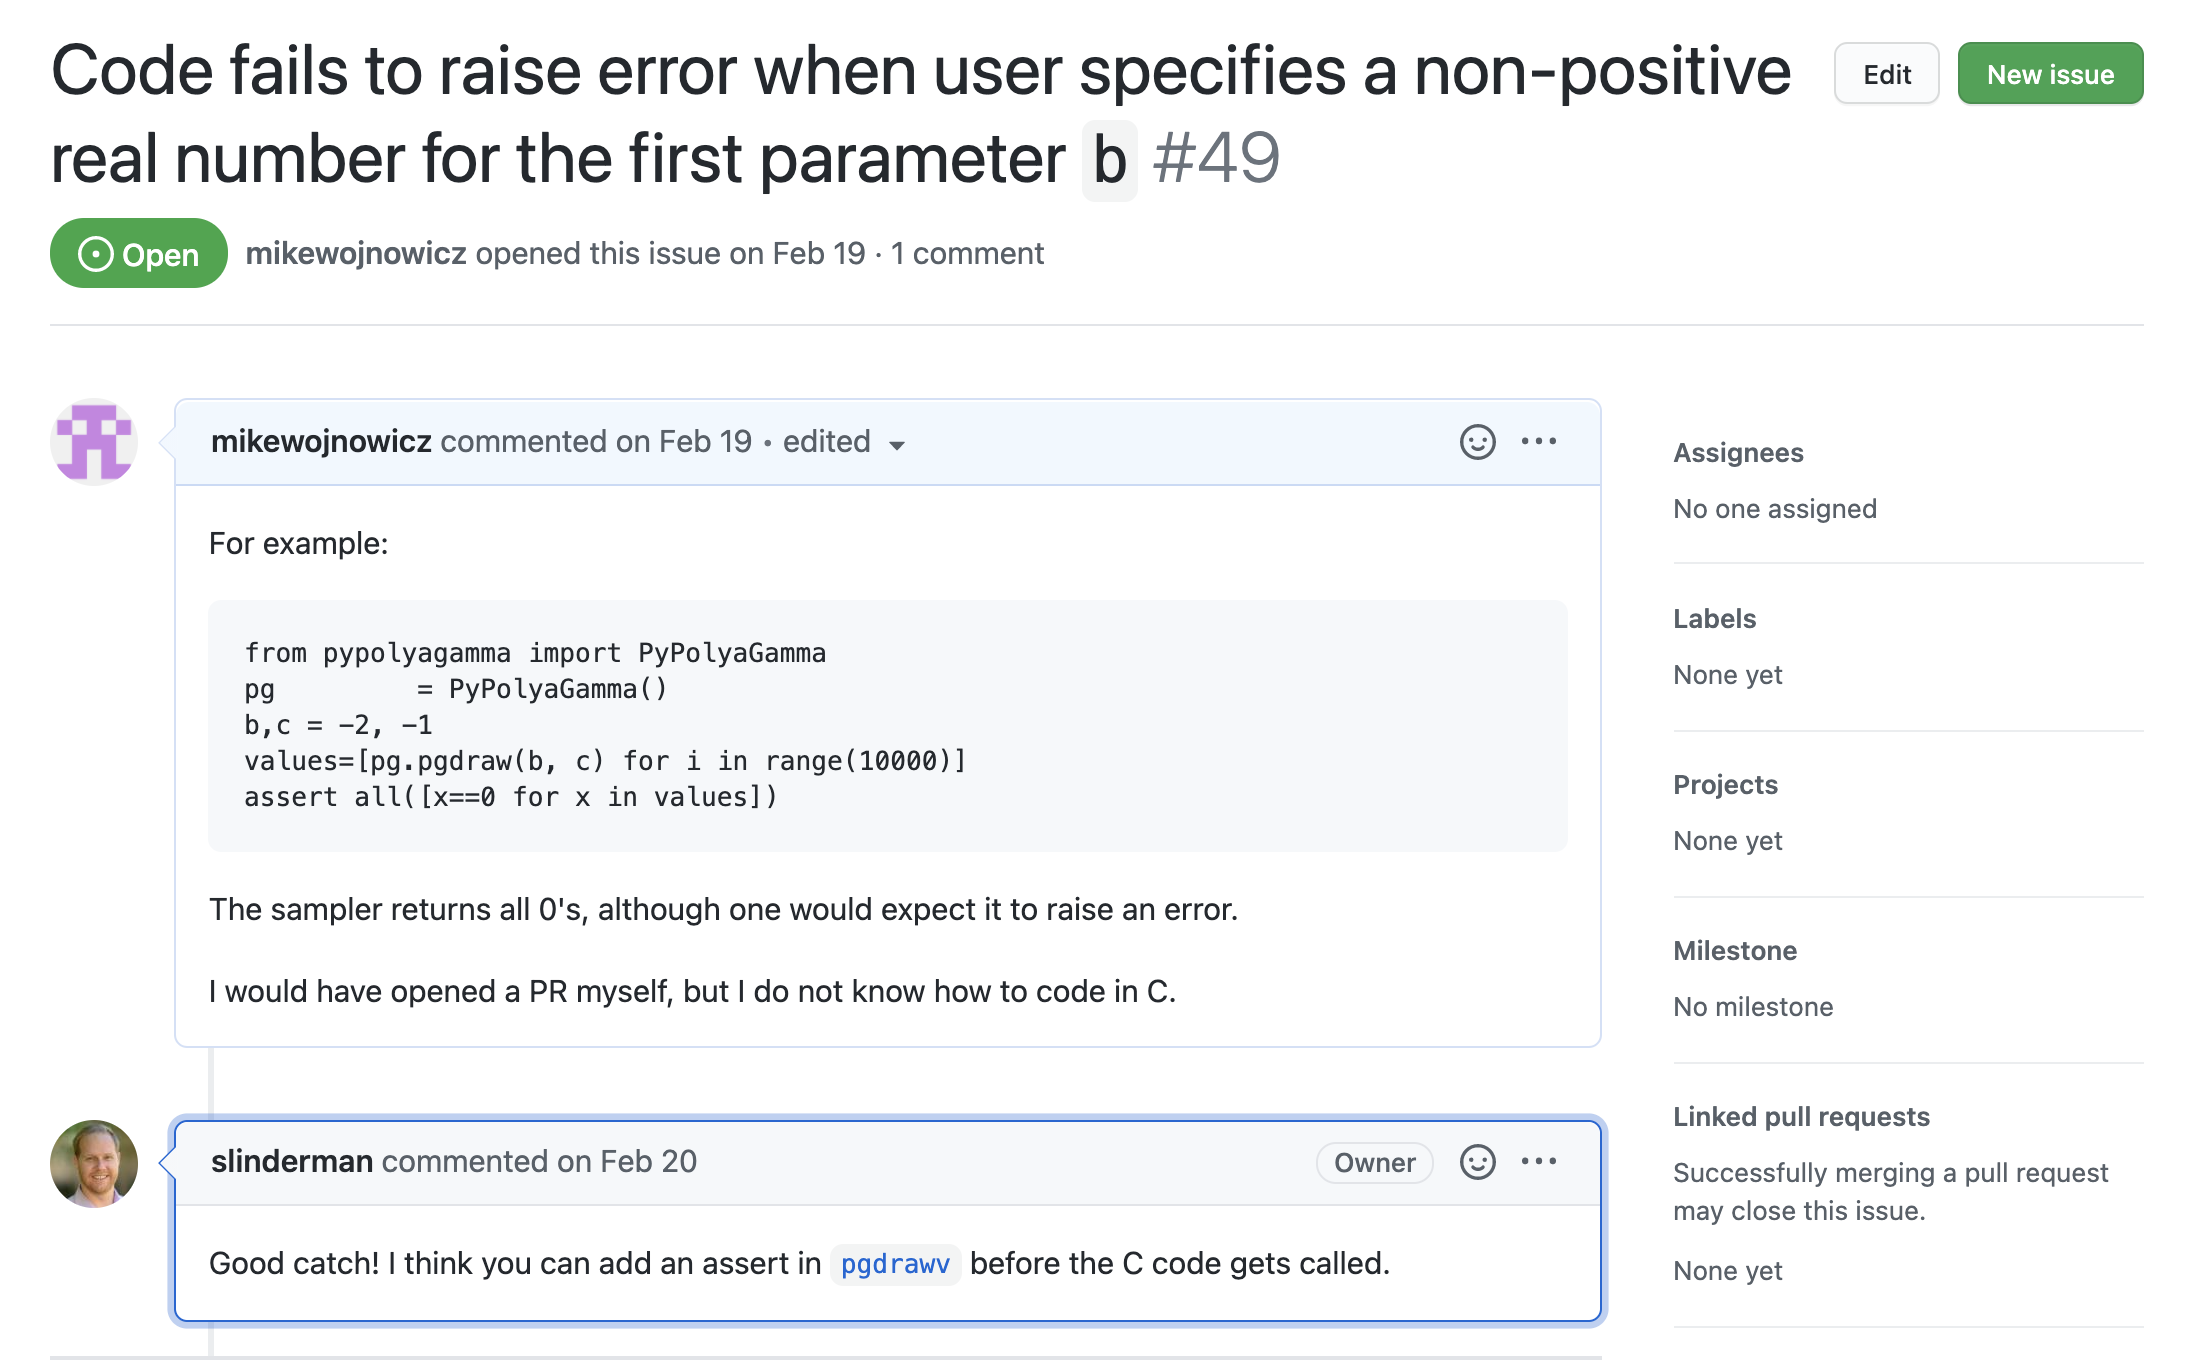
\includegraphics[width=\textwidth]{images/pypolyagamma_issue}	
\end{center}
	
\end{frame}

\section{Good practices}
\begin{frame}{Some good practices}

\begin{itemize}
\item Should be \alert{fast} (5-10 seconds to run \textit{all} tests).
\item Run tests before committing changes to source code. 
\item Each test function name should have a postfix describing what we're testing:
	\begin{center}\url{test__function_name__what_property_we_are_testing}	
	\end{center}
\item One assertion per test.
\end{itemize} 
\end{frame}



\end{document}